% ============================================================
% 第六章 系统集成与车载使用场景设计
% ============================================================

\chapter{系统集成与车载使用场景设计}

\section{系统集成概述}

\subsection{系统总体架构}

飞行雨伞系统由四个相互独立又协同工作的子系统构成，
如表~\ref{tab:subsystem_overview}所示。

\begin{longtable}{p{3.2cm} p{5.0cm} p{5.5cm}}
    \caption{飞行雨伞系统子系统构成}
    \label{tab:subsystem_overview} \\

    % -------- 第一页表头 --------
    \toprule
    子系统 & 核心组件 & 功能定位 \\
    \midrule
    \endfirsthead

    % -------- 续页表头 --------
    \multicolumn{3}{l}{\small 续表~\ref*{tab:subsystem_overview}} \\[2pt]
    \toprule
    子系统 & 核心组件 & 功能定位 \\
    \midrule
    \endhead

    % -------- 每页底部（非末页）--------
    \midrule
    \multicolumn{3}{r}{\small 接下页} \\
    \endfoot

    % -------- 最后一页底部 --------
    \bottomrule
    \endlastfoot

    % -------- 表格内容 --------
    充气伞体系统
        & 气柱骨架、TPU伞面、PLA节点、充气阀
        & 形态重构载体，实现收纳$\leftrightarrow$飞行形态切换 \\[6pt]
    多旋翼动力系统
        & 电机$\times$4、ESC$\times$4、桨叶$\times$4、电池
        & 提供飞行升力，实现姿态与位置控制 \\[6pt]
    嵌入式飞行控制系统
        & Pixhawk 6C、IMU、气压计、GPS
        & 传感器融合、姿态估计与控制律解算 \\[6pt]
    车载平台系统
        & 车载充气泵、遥控器、地面电源、收纳袋
        & 提供充气、控制与能源支持，实现车载集成 \\


\end{longtable}
\FloatBarrier 
飞行雨伞系统的整机集成（收纳）形态如图~\ref{fig:drone_cad}所示，
四个旋翼单元通过气柱骨架与正方形中心框架连接，
飞控（绿色）安装于中心框架顶部，整体结构紧凑对称。

\begin{figure}[htbp]
    \centering
    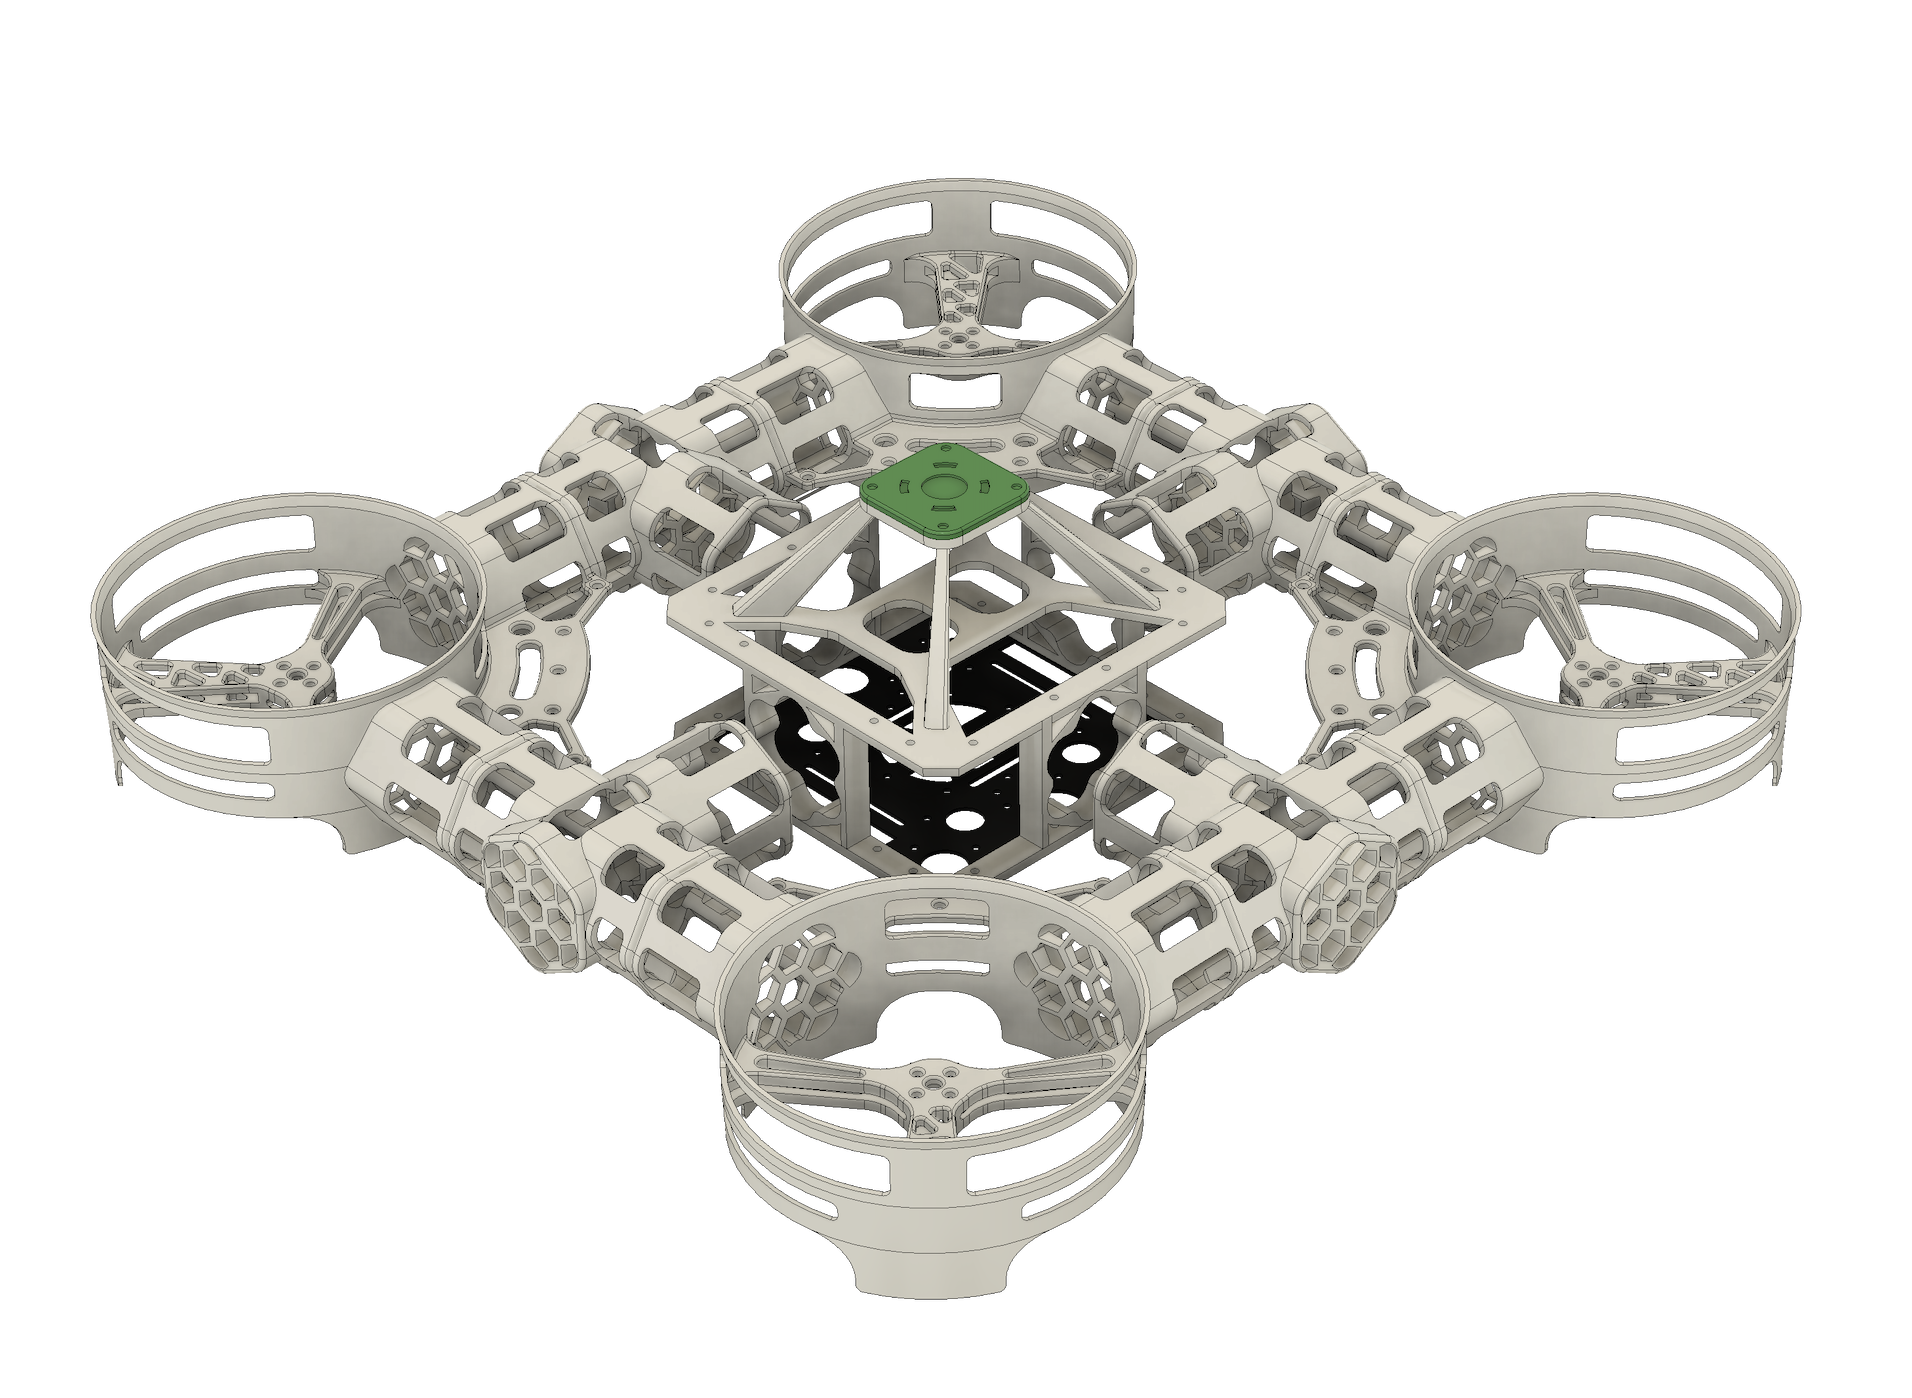
\includegraphics[width=0.35\textwidth]{figures/fig6_drone_cad.png}
    \caption{飞行雨伞系统收纳态CAD渲染图}
    \label{fig:drone_cad}
\end{figure}
\FloatBarrier

\subsection{电子系统集成架构}

动力飞行子系统的电子集成采用标准多旋翼架构，信号与电源流如下：

\textbf{遥控信号链路}：乐迪AT9S Pro（9通道，2.4\,GHz FHSS）
$\rightarrow$ R9DS接收机 $\rightarrow$ Pixhawk 6C（SBUS协议）

\textbf{控制输出链路}：Pixhawk 6C $\rightarrow$ ESC$\times$4（PWM协议）
$\rightarrow$ 无刷电机$\times$4

\textbf{传感回路}：IMU（内置）+ 气压计（内置）+ GPS（外置，UART接口）
$\rightarrow$ Pixhawk 6C状态估计器

飞控安装于骨架中心平台，GPS模块固定于飞控上方伞面固定架，
远离电机以减少电磁干扰。
四个ESC沿骨架气柱布线，通过扎带固定于对应气柱外侧，
保持整体布局的重心对称性。


\section{收纳态设计}

\subsection{收纳形态特征}

充气结构子系统的核心设计价值之一，在于实现从"飞行器"到"随身携带物品"的形态降维。
当气柱骨架完全排气后，整个系统折叠为厚度约3$\sim$5\,cm的扁平形态，
平面尺寸与一台笔记本电脑相当。

如图~\ref{fig:concept_render}所示，收纳态的飞行雨伞外形圆润紧凑，
整机起飞质量约 1.68\,kg（含机载电池），可单手持握，或置于专属收纳袋中存放于车辆后备箱、
座椅背后等空间。
这一形态特征从根本上消除了传统无人机"体积庞大、不便携带"的使用痛点，
使飞行雨伞真正具备随车常备的可行性。


\begin{figure}[htbp]
    \centering
    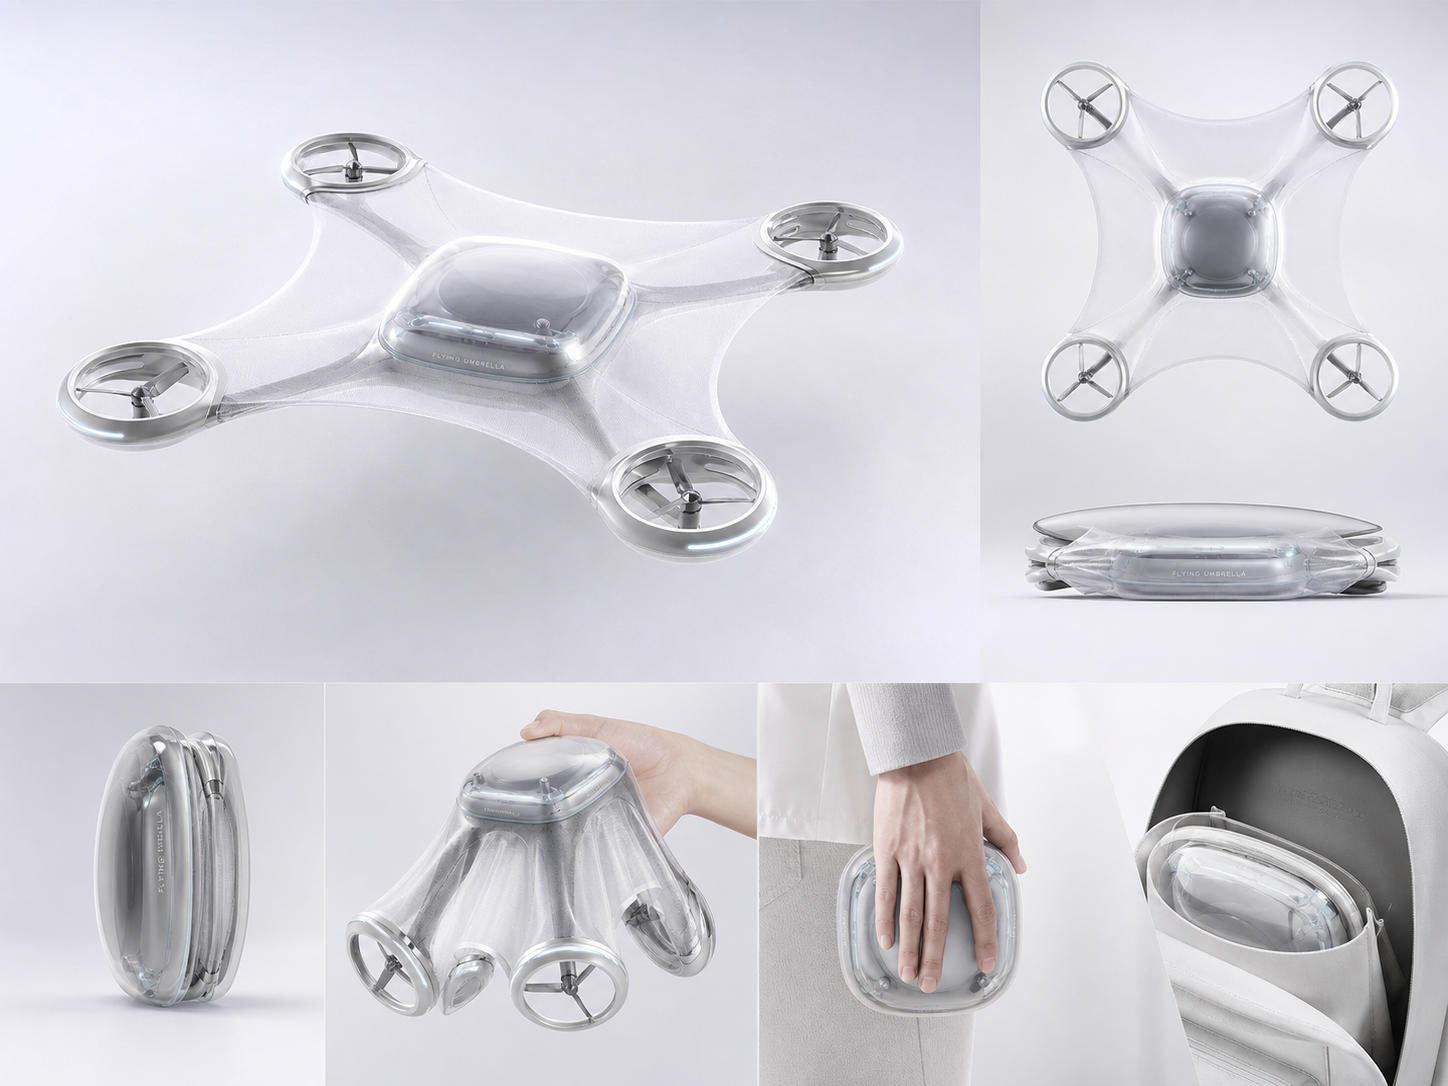
\includegraphics[width=0.75\textwidth]{figures/fig6_1_concept_render.png}
    \caption{飞行雨伞系统收纳态与飞行态概念效果图}
    \label{fig:concept_render}
\end{figure}
\FloatBarrier 

\subsection{收纳操作流程}

从飞行态到收纳态的转换操作步骤如下：

\begin{enumerate}
    \item 飞行雨伞完成飞行任务，操控降落至地面；
    \item 关闭电机，确认系统安全停机；
    \item 打开充气阀放气口，气柱在大气压差作用下自然排气；
    \item 配合手动辅助按压加速排气过程（约10$\sim$20\,s完成）；
    \item 将排气后的扁平结构折叠收纳，放入收纳袋归位。
\end{enumerate}

整个收纳操作无需工具，由单人即可完成，预计操作时间不超过60\,s。


\section{车载部署方案设计}

\subsection{车载存放方案}

飞行雨伞的车载存放依托新能源汽车后备箱空间实现。
收纳态系统置于专属收纳袋，与车载充气泵、遥控器等配件一同存放于后备箱，
不占用乘坐空间，亦不影响日常用车。

收纳袋设计需满足以下要求：防水材质（应对雨天取用场景）；
有一定保护衬垫（防止气柱在车辆行驶振动中磨损）；
开合方便（单手可操作）。
收纳袋通过魔术贴或弹性绑带固定于后备箱侧壁或底板，
防止车辆行驶时滑移，适配市售大多数SUV和轿车车型，
无需对车辆进行任何改造。

\subsection{充气展开方案}

车载充气泵采用12\,V直流微型充气泵，
通过车辆点烟器接口或12\,V车载电源接口供电，无需额外电源设备。
充气时，将充气泵气嘴对接飞行雨伞骨架上的充气阀接口，开启充气泵即可。

充气过程中，骨架气柱和伞面气柱依次充气，
系统从扁平收纳态逐渐展开为正方形飞行形态。
充气完成时间约30$\sim$60\,s（取决于充气泵额定流量）。
充气完成后，充气阀自动密封，断开充气泵接口即可准备起飞。

\subsection{起降平台设计考量}

在当前样机阶段，飞行雨伞的起飞与降落地点为车辆附近的平整地面，
无需专属停机坪。系统充气展开并完成飞控上电校准后，
从地面垂直起飞，上升至设计工作高度（$2.0\sim2.5$\,m）后进入悬停遮雨模式。

在更进一步的产品化设计构想中，
起降平台可集成于后备箱开口处（如图~\ref{fig:concept_render}效果图所示），
充气展开、起飞、降落、排气收纳的全流程均在后备箱开口前方完成，
实现更高程度的自动化与一体化。
这一构型在当前样机阶段不作为工程实现目标，
作为未来产品迭代方向在此记录。


\section{完整使用流程设计}
基于以上各子系统设计，结合第二章所定义的六阶段使用流程，
飞行雨伞的完整操作步骤可细化为以下八步，


\begin{enumerate}
    \item \textbf{车辆抵达目的地}，停车；
    \item \textbf{打开后备箱}，取出收纳态飞行雨伞；
    \item \textbf{连接12\,V车载充气泵}，对接充气阀，启动充气泵；
    \item \textbf{等待30$\sim$60\,s充气展开}，确认骨架完全撑开；
    \item \textbf{开启遥控器和飞控}，等待GPS定位锁定（约30\,s）；
    \item \textbf{推油门起飞}，上升至工作高度$2.0\sim2.5$\,m；
    \item \textbf{遮雨服务阶段}：操作者手持遥控器跟随用户，
          控制飞行雨伞悬停于用户头顶上方；
    \item \textbf{任务完成}，降落→关机→排气收纳，归位后备箱。
\end{enumerate}

从取出到完成起飞的\textbf{准备时间约90\,s}
（充气60\,s + 飞控启动及GPS锁定30\,s），
从降落到完成收纳的\textbf{收纳时间约60\,s}。


\section{通信与控制链路}

\subsection{遥控器系统}

本系统使用\textbf{乐迪AT9S Pro}遥控器（9通道，2.4\,GHz FHSS跳频扩频技术），
控制半径可达1.5\,km，远超本系统最大飞行距离（用户周边5\,m范围内），
通信可靠性充裕。

在实际使用中，操作者手持遥控器跟随用户步行，
通过遥控器实时控制飞行雨伞的位置与高度，
使悬停中心始终对准用户头顶上方。
这一"操作者跟随"模式是本阶段样机的主要工作方式。
全自主视觉跟随功能（基于摄像头目标检测与跟踪）
作为后续研究方向，不在本文实现范围之内。

\subsection{飞行安全机制}

乐迪AT9S Pro 具备失控保护（Failsafe）特性。当遥控信号连续丢失大于0.5s的时候，飞控就会启动预设的失控处理逻辑，执行原地降落，防止飞行器继续漂移或者拉高。
本系统的最大飞行高度为2m以内，所以失控保护主要针对低空环境进行设计。在此工作范围之内，飞行器即使出现遥控中断的情况，也能较快地完成飞行任务，把人员所受的风险控制在较小的范围内。
除此之外，在系留供电模式下，长约150cm的系留缆线自身就存在物理上的约束。即使电子失控保护没有完全起作用，缆线仍然可以作为机械上的备用，在功能验证的时候提高测试的安全性。


\section{本章小结}

本章完成飞行雨伞系统集成架构的设计以及车载使用场景的规划。系统由充气伞体、多旋翼动力、嵌入式飞行控制和车载平台四个子系统组成，各个部分用标准接口配合工作。

收纳态设计使系统具有了随车携带、随时部署的特点。其收纳体积约为一台笔记本电脑，单人60s内可以完成收纳或者展开。

车载部署方案使用的是12V车载电源，不需要对车辆做任何改装。从取出到起飞完整的操作时间大约为 90s，普通用户可以完成大部分的操作。

通信链路采用乐迪AT9S Pro遥控器，飞控核心为 Pixhawk~6C。低空（$\leq 2$\,m）工作时，失控保护和系留缆线约束一起成为目前的安全措施。

目前系统仍然使用操作者手动遥控的方式进行跟随，用户自主跟随的功能还没有实现；全自主视觉跟随还要继续研究。